% Research paper (anonymized) focused solely on skyline/Pareto mathematics.
% Author: Emily Montes
\documentclass[11pt]{article}

\usepackage[margin=1in]{geometry}
\usepackage{amsmath, amssymb, amsthm}
\usepackage{graphicx}
\usepackage{booktabs}
\usepackage{hyperref}
\usepackage{microtype}

% Optional (nice figures). If your TeX install lacks pgfplots/tikz, comment this block.
\usepackage{tikz}
\usepackage{pgfplots}
\pgfplotsset{compat=1.18}

\title{Exact Skyline Reduction for Monotone Scoring in Rhythm-Game Loadout Optimization}
\author{Emily Montes}
\date{April 2026}

\theoremstyle{plain}
\newtheorem{theorem}{Theorem}
\newtheorem{lemma}{Lemma}
\newtheorem{corollary}{Corollary}
\newtheorem{definition}{Definition}

\begin{document}
\maketitle

\begin{abstract}
Skyline (Pareto-frontier) reduction is a mathematically exact technique for eliminating impossible winners in optimization problems whose objective is monotone in a chosen coordinate system. This paper formalizes the skyline principle and shows why it provides \emph{exactness} rather than heuristic improvement for a family of rhythm-game scoring models that depend on discrete stat indices and elemental values. We present (i) a general monotone-optimum-on-the-skyline theorem, (ii) conditions required for skyline exactness (sufficiency and monotonicity), and (iii) a concrete skyline application over loadout signatures. We emphasize correctness: skyline pruning discards only states that are provably dominated under the exact score semantics.
\end{abstract}

\section{Problem statement}
We consider a rhythm game in which a player selects a \emph{loadout} (equipment + minis) and then distributes a limited integer \emph{gem budget} across several upgrade stats. The score of a chart is computed deterministically from:
\begin{itemize}
  \item A fixed chart structure (note timestamps, note types, and a fixed \emph{fever} activation logic).
  \item Discrete stat indices controlling multipliers: \emph{Perfect Points} (PP), \emph{Combo Multiplier} (CM), \emph{Fever Multiplier} (FM), \emph{Fever Time} (FT), \emph{Fever Fill Rate} (FF).
  \item Elemental values over the set of elementals
  \[ \mathcal{E} = \{\text{Chill},\,\text{Flow},\,\text{Rush},\,\text{Beat},\,\text{Vibe}\}. \]
  Each loadout has a \emph{primary} elemental $P\in\mathcal{E}$ and \emph{secondary} elemental $S\in\mathcal{E}$.
  \item A selectable \emph{Elemental} gem type that increases the chosen elemental (the \emph{selected elemental}) and contributes to the base score through that elemental value.
\end{itemize}

The global objective is:
\begin{quote}
\emph{Find the (loadout, gem-allocation) pair that maximizes the exact in-game score.}
\end{quote}

The raw search space is combinatorial (many equipment combinations and many integer allocations). Skyline mathematics enters as an \emph{exact reduction}: it discards candidates that cannot be optimal under provable dominance.

\section{Skyline preliminaries}

\subsection{Partial order and dominance}
\begin{definition}[Product order]
For vectors $x,y\in\mathbb{R}^d$, define $x\preceq y$ if $x_i\le y_i$ for all coordinates $i=1,\dots,d$. Define strict dominance $x\prec y$ if $x\preceq y$ and $x\neq y$.
\end{definition}

\begin{definition}[Skyline / Pareto frontier]
Given a finite set $X\subset\mathbb{R}^d$, the skyline is
\[
\mathrm{Skyline}(X) = \{x\in X : \nexists\,y\in X\text{ with } x\prec y\}.
\]
Equivalently, $x$ is on the skyline if it is not strictly dominated by any other point.
\end{definition}

\subsection{Monotone objectives imply skyline optimality}
\begin{definition}[Coordinate-wise monotonicity]
A function $f:\mathbb{R}^d\to\mathbb{R}$ is (weakly) monotone if
\[ x\preceq y \implies f(x)\le f(y). \]
\end{definition}

\begin{theorem}[Optimum lies on the skyline]
\label{thm:skyline-opt}
Let $X\subset\mathbb{R}^d$ be finite and let $f$ be monotone. Then
\[
\max_{x\in X} f(x) \;=\; \max_{x\in \mathrm{Skyline}(X)} f(x).
\]
\end{theorem}

\begin{proof}
Let $x^*\in\arg\max_{x\in X} f(x)$. If $x^*\in\mathrm{Skyline}(X)$ we are done. Otherwise there exists $y\in X$ such that $x^*\prec y$. By monotonicity, $f(y)\ge f(x^*)$, so $y$ is also optimal. If $y$ is not on the skyline, repeat the argument. Because $X$ is finite and strict dominance cannot loop, this process terminates at a skyline point $\bar{x}$ with $f(\bar{x})=\max_{x\in X} f(x)$. Hence the maxima are equal.
\end{proof}

\paragraph{Interpretation.} Skyline is not an approximation: it is the smallest subset that preserves \emph{all} maxima of \emph{all} monotone functions defined on the coordinates.

\section{Score structure and the monotonicity requirement}
Skyline exactness requires selecting coordinates that make the \emph{exact score} monotone.

\subsection{A score-relevant coordinate system}
We will use the outer loadout signature as the primary example; the inner $(B, C, F)$ tuple is introduced only to state the monotonicity conditions that make skyline exact.

\paragraph{Outer signature coordinates.}
A loadout induces a base signature vector
\[
\sigma = (\mathrm{PP},\,\mathrm{CM},\,\mathrm{FM},\,\mathrm{FT},\,\mathrm{FF},\,B_{\mathrm{lane}})\in\mathbb{Z}^6,
\]
where $B_{\mathrm{lane}}$ is the scalar ``lane base'' term
\[
B_{\mathrm{lane}} \;:=\; 2\,v_P + v_S,
\]
and $v_P,v_S$ are the primary and secondary elemental values produced by the loadout (after applying equipment and minis, but before spending gems).

\paragraph{Inner outcome coordinates.}
Fix a chart and fix an FT/FF choice, which fixes a fever/non-fever pattern over notes (a \emph{timeline mask}). For a fixed loadout and a fixed remaining gem budget, a gem allocation induces three scalars:
\[
\tau = (B,\,C,\,F)\in\mathbb{R}_{\ge 0}\times\mathbb{R}_{\ge 1}\times\mathbb{R}_{\ge 1},
\]
where:
\begin{itemize}
  \item $B$ is the base value (a function of $B_{\mathrm{lane}}$, PP effects, and elemental contributions),
  \item $C$ is the combo multiplier (determined by the CM index),
  \item $F$ is the fever multiplier (determined by the FM index).
\end{itemize}

\subsection{Why monotonicity holds in this model}
The skyline proofs require: if $(B,C,F)\preceq (B',C',F')$ then the exact score under the fixed timeline mask does not decrease.

The only subtlety is that the exact score is typically a sum of per-note integer truncations. The following lemma is the core fact.

\begin{lemma}[Monotonicity survives per-note truncation]
\label{lem:floor-monotone}
Let $g(t)$ be a nondecreasing real-valued function and define $h(t)=\lfloor g(t)\rfloor$. Then $h(t)$ is nondecreasing.
\end{lemma}
\begin{proof}
If $t\le t'$ then $g(t)\le g(t')$. Applying floor preserves order: $\lfloor g(t)\rfloor\le\lfloor g(t')\rfloor$.
\end{proof}

\begin{corollary}[Monotone score in $(B,C,F)$]
\label{cor:monotone-bcf}
Assume each note contribution is of the form $\lfloor \alpha(B,C)\cdot m(F) \rfloor$ where $\alpha$ is nondecreasing in both $B$ and $C$ and $m$ is nondecreasing in $F$ with $m(F)\ge 0$. Then the total exact score (a finite sum over notes) is nondecreasing in $B$, $C$, and $F$.
\end{corollary}

\paragraph{Key point.} Once exact monotonicity is established for a coordinate system, Theorem~\ref{thm:skyline-opt} applies automatically.

\section{Skyline as an exact reduction}

\subsection{Outer skyline: nondominated loadout signatures}
Let $\Sigma$ be the set of all achievable outer signatures $\sigma$ from all legal loadouts.

If the exact score is nondecreasing in each coordinate of $\sigma$ (PP, CM, FM, FT, FF, and $B_{\mathrm{lane}}$), then by Theorem~\ref{thm:skyline-opt}:
\[
\max_{\sigma\in\Sigma} \mathrm{Score}(\sigma) 
\;=\;
\max_{\sigma\in\mathrm{Skyline}(\Sigma)} \mathrm{Score}(\sigma).
\]

\paragraph{Meaning.} Any loadout signature dominated by another signature is an \emph{impossible winner}. It can be deleted without changing the optimal achievable score.

\paragraph{Generalization.} The same theorem applies to any candidate family whose exact score is monotone in a score-sufficient coordinate system; the outer loadout skyline is the paper's concrete instance.

\section{Illustrations}

\subsection{A 2D skyline example}
Figure~\ref{fig:2d-skyline} shows a classic skyline: points represent candidates; gray points are dominated; red points form the skyline.

\begin{figure}[ht]
\centering
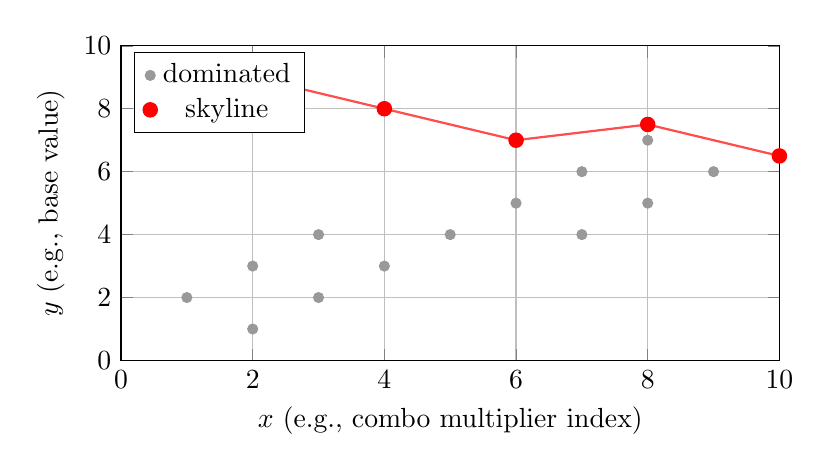
\begin{tikzpicture}
\begin{axis}[
  width=0.82\linewidth,
  height=0.46\linewidth,
  xlabel={$x$ (e.g., combo multiplier index)},
  ylabel={$y$ (e.g., base value)},
  xmin=0, xmax=10,
  ymin=0, ymax=10,
  grid=both,
  legend style={at={(0.02,0.98)},anchor=north west},
]

% Dominated points
\addplot[only marks, mark=*, mark size=1.8pt, color=black!40] coordinates {
  (1,2) (2,1) (2,3) (3,2) (3,4) (4,3) (5,4) (6,5) (7,4) (7,6)
  (8,5) (8,7) (9,6)
};
\addlegendentry{dominated}

% Skyline points (manually chosen for illustration)
\addplot[only marks, mark=*, mark size=2.6pt, color=red] coordinates {
  (2,9) (4,8) (6,7) (8,7.5) (10,6.5)
};
\addlegendentry{skyline}

% A simple frontier polyline
\addplot[no marks, color=red!70, thick] coordinates {
  (2,9) (4,8) (6,7) (8,7.5) (10,6.5)
};

\end{axis}
\end{tikzpicture}
\caption{A 2D skyline. If an objective is monotone in $(x,y)$, an optimum must occur at a skyline point.}
\label{fig:2d-skyline}
\end{figure}

\subsection{Why skyline is ``exact,'' not heuristic}
Skyline does not guess which points are bad. It applies a logical implication:
\[
(x\prec y) \wedge (f\text{ monotone}) \implies f(x)\le f(y).
\]
Therefore removing $x$ cannot remove the maximizer.

\section{Exactness conditions and common pitfalls}
Skyline exactness is conditional on two requirements.

\paragraph{(1) Monotonicity.} If any coordinate can increase while the exact score decreases (a non-monotone mechanic), dominance pruning can fail.

\paragraph{(2) Sufficiency of coordinates.} The skyline must be computed in a coordinate system that fully determines the exact score. If a hidden variable affects scoring but is not included, two candidates can appear ordered in the reduced space while their true scores do not respect that order.

\section{Conclusion}
Skyline reduction is a rigorous method for exact optimization under monotone scoring: it deletes only candidates that are provably dominated. In rhythm-game loadout optimization, the outer skyline over loadout signatures is an exact reduction of the search space. More generally, the same proof pattern applies whenever the chosen coordinates are score-sufficient and the exact objective is coordinate-wise monotone.

\begin{thebibliography}{9}
\bibitem{pareto}
V. Pareto, \emph{Cours d'\'economie politique}. Lausanne, 1896.

\bibitem{skyline-db}
S. B\"orzs\"onyi, D. Kossmann, and K. Stocker, ``The skyline operator,'' \emph{Proceedings of the 17th International Conference on Data Engineering}, 2001.
\end{thebibliography}

\end{document}
